% ch06 译文：原文 §4a 后半、§4b、§4c、§4d（main.tex 第 1192--1478 行）
% 边界说明：为保持例与 figure 环境完整，本块自 p.24 上的 \begin{exmp} 起收（含整幅图 4）；
%   p.24 页首标记在前块 ch05。页首标记按 work/pagemarks/ch06.txt，仅标 p.25--p.30。
% 注：下文 tikzcd 图沿用源文的引号标签（ASCII 双引号包住 \simeq），需 tikz 的 quotes 库。
\usetikzlibrary{quotes}

\begin{exmp}\label{exmp:wrapped-Fukaya-cat-twice-punctured-equivariant}
    作为另一个例子，我们构造 Weinstein 扇形 $(\mathbb{C}\setminus\{\pm 1\},2/(1-z^2))$ 的 $\mathbb{Z}^2$-覆盖 $\mathcal{X}$。该 Weinstein 扇形可看作两个 Weinstein 扇形 $\left(\mathbb{C}^{\ast},z+z^{-1}\right)$ 沿其中一个边界停止位的扇形粘合（sectorial gluing），其 $\mathbb{Z}^2$-覆盖则可实现为每个扇形的 $\mathbb{Z}$ 个副本沿 $\mathbb{Z}^2$ 个条带粘合，如图 \ref{fig:Z2-cover-twice-punctured-disk} 所示。\par
    \begin{figure}[ht]
        \centering
        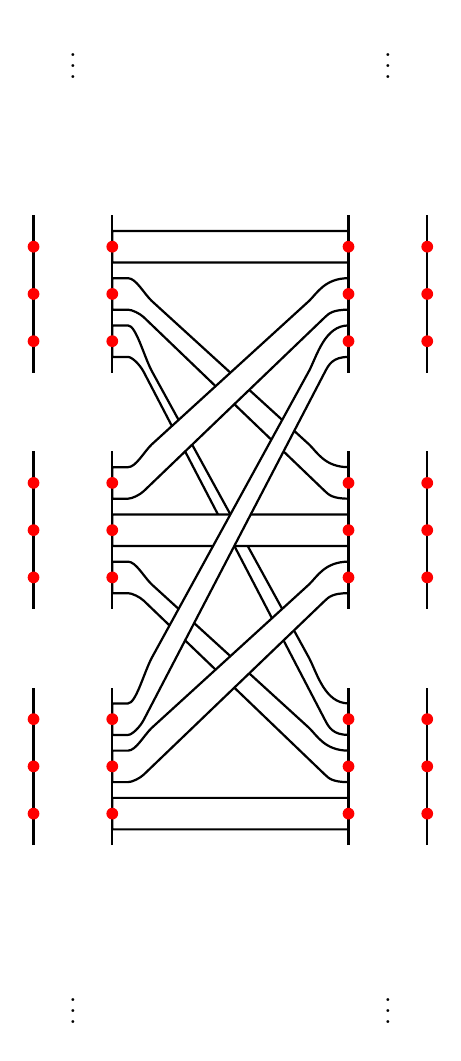
\begin{tikzpicture}       
        \begin{scope}[yshift=6cm]
            \draw [thick] (0,0) -- (0,2);
            \draw [thick] (1,0) -- (1,2);
                \foreach \x in {0.2,0.8,1.4}{
                \filldraw [fill=white, draw=black,thick] (1,\x)
            -- (1.2,\x)
            .. controls (1.25,\x)
                       and (1.35,{0.98*\x+0.02*((\x-0.2)/0.2-4.6)})
            .. (1.4,{0.96*\x+0.04*((\x-0.2)/0.2-4.6)})
            -- (3.7,{0.04*\x+0.96*((\x-0.2)/0.2-4.6)})
            .. controls (3.75,{0.02*\x+0.98*((\x-0.2)/0.2-4.6)})
                       and (3.8,{(\x-0.2)/0.2-4.6})
            .. (4,{(\x-0.2)/0.2-4.6}) -- (4,{(\x-0.2)/0.2 -4.2})
            .. controls (3.7,{(\x-0.2)/0.2-4.2}) and (3.6,{((\x-0.2)/0.2-4.2)-0.2*((\x-0.2)/0.2-4.6-\x)/2.5})
            .. (3.5,{((\x-0.2)/0.2-4.2)-0.3*((\x-0.2)/0.2-4.6-\x)/2.5})
            -- (1.5,{\x+0.4+0.3*((\x-0.2)/0.2-4.6-\x)/2.5})
            .. controls (1.4,{\x+0.4+0.2*((\x-0.2)/0.2-4.6-\x)/2.5}) and (1.3,{\x+0.4})
            ..(1.2,{\x+0.4}) -- (1,{\x+0.4}) -- cycle;
            }
            \foreach \x in {0.4,1,1.6} {
                \node [circle,fill=red,inner sep=1.5pt] at (0,\x) {};
                \node [circle,fill=red,inner sep=1.5pt] at (1,\x) {};
            }
        \end{scope}
        \begin{scope}[yshift=3cm]
            \draw [thick] (0,0) -- (0,2);
            \draw [thick] (1,0) -- (1,2);
            \foreach \x in {0.2,0.8,1.4}{
                \filldraw [fill=white, draw=black, thick] (1,\x)
            -- (1.2,\x)
            .. controls (1.25,\x)
                       and (1.35,{0.98*\x+0.02*((\x-0.2)/0.2-2.2)})
            .. (1.4,{0.96*\x+0.04*((\x-0.2)/0.2-2.2)})
            -- (3.7,{0.04*\x+0.96*((\x-0.2)/0.2-2.2)})
            .. controls (3.75,{0.02*\x+0.98*((\x-0.2)/0.2-2.2)})
                       and (3.8,{(\x-0.2)/0.2-2.2})
            .. (4,{(\x-0.2)/0.2-2.2}) -- (4,{(\x-0.2)/0.2 -1.8})
            .. controls (3.7,{(\x-0.2)/0.2-1.8}) and (3.6,{((\x-0.2)/0.2-1.8)-0.2*((\x-0.2)/0.2-2.2-\x)/2.5})
            .. (3.5,{((\x-0.2)/0.2-1.8)-0.3*((\x-0.2)/0.2-2.2-\x)/2.5})
            -- (1.5,{\x+0.4+0.3*((\x-0.2)/0.2-2.2-\x)/2.5})
            .. controls (1.4,{\x+0.4+0.2*((\x-0.2)/0.2-2.2-\x)/2.5}) and (1.3,{\x+0.4})
            ..(1.2,{\x+0.4}) -- (1,{\x+0.4}) -- cycle;
            }
            \foreach \x in {0.4,1,1.6} {
                \node [circle,fill=red,inner sep=1.5pt] at (0,\x) {};
                \node [circle,fill=red,inner sep=1.5pt] at (1,\x) {};
            }
        \end{scope}
        \begin{scope}
            \draw [thick] (0,0) -- (0,2);
            \draw [thick] (1,0) -- (1,2);
            \foreach \x in {0.2,0.8,1.4}{
                \filldraw [fill=white, draw=black,thick] (1,\x)
            -- (1.2,\x)
            .. controls (1.25,\x)
                       and (1.35,{0.98*\x+0.02*((\x-0.2)/0.2+0.2)})
            .. (1.4,{0.96*\x+0.04*((\x-0.2)/0.2+0.2)})
            -- (3.7,{0.04*\x+0.96*((\x-0.2)/0.2+0.2)})
            .. controls (3.75,{0.02*\x+0.98*((\x-0.2)/0.2+0.2)})
                       and (3.8,{(\x-0.2)/0.2+0.2})
            .. (4,{(\x-0.2)/0.2+0.2}) -- (4,{(\x-0.2)/0.2 +0.6})
            .. controls (3.7,{(\x-0.2)/0.2+0.6}) and (3.6,{((\x-0.2)/0.2+0.6)-0.2*((\x-0.2)/0.2+0.2-\x)/2.5})
            .. (3.5,{((\x-0.2)/0.2+0.6)-0.3*((\x-0.2)/0.2+0.2-\x)/2.5})
            -- (1.5,{\x+0.4+0.3*((\x-0.2)/0.2+0.2-\x)/2.5})
            .. controls (1.4,{\x+0.4+0.2*((\x-0.2)/0.2+0.2-\x)/2.5}) and (1.3,{\x+0.4})
            ..(1.2,{\x+0.4}) -- (1,{\x+0.4}) -- cycle;
            }
            \foreach \x in {0.4,1,1.6} {
                \node [circle,fill=red,inner sep=1.5pt] at (0,\x) {};
                \node [circle,fill=red,inner sep=1.5pt] at (1,\x) {};
            }
        \end{scope}
        \begin{scope}[yshift=3cm, xshift=4cm]
            \draw [thick] (0,0) -- (0,2);
            \draw [thick] (1,0) -- (1,2);
            \foreach \x in {0.4,1,1.6} {
                \node [circle,fill=red,inner sep=1.5pt] at (0,\x) {};
                \node [circle,fill=red,inner sep=1.5pt] at (1,\x) {};
            }
        \end{scope}     
        \begin{scope}[xshift=4cm]
            \draw [thick] (0,0) -- (0,2);
            \draw [thick] (1,0) -- (1,2);
            \foreach \x in {0.4,1,1.6} {
                \node [circle,fill=red,inner sep=1.5pt] at (0,\x) {};
                \node [circle,fill=red,inner sep=1.5pt] at (1,\x) {};
            }
        \end{scope}
        \begin{scope}[yshift=6cm,xshift=4cm]
            \draw [thick] (0,0) -- (0,2);
            \draw [thick] (1,0) -- (1,2);
            \foreach \x in {0.4,1,1.6} {
                \node [circle,fill=red,inner sep=1.5pt] at (0,\x) {};
                \node [circle,fill=red,inner sep=1.5pt] at (1,\x) {};
            }
        \end{scope}
        \begin{scope}[yshift=9cm]
            \node at (0.5,1) {$\vdots$};
        \end{scope}
        \begin{scope}[yshift=-3cm]
            \node at (0.5,1) {$\vdots$};
        \end{scope}
        \begin{scope}[yshift=9cm,xshift=4cm]
            \node at (0.5,1) {$\vdots$};
        \end{scope}
        \begin{scope}[yshift=-3cm,xshift=4cm]
            \node at (0.5,1) {$\vdots$};
        \end{scope}
        \end{tikzpicture}
    \caption{$\mathbb{Z}^2$-cover of the Twice-Punctured Disk with Stops.}\label{fig:Z2-cover-twice-punctured-disk}
    \end{figure}
% [原文 p.25]
    由于已知此粘合中每个扇形的生成元，对图表
\[
        \begin{tikzcd}
            \mathcal{W} \left(\bigsqcup_{\mathbb{Z}^2}T^{\ast}[0,1]\right)\arrow[r]\arrow[d]&\mathcal{W} \left(\bigsqcup_{\mathbb{Z}}(\mathbb{C},e^{z_1}+e^{-z_1})\right)\\ 
            \mathcal{W}\left(\bigsqcup_{\mathbb{Z}}(\mathbb{C},e^{z_2}+e^{-z_2})\right)&
        \end{tikzcd}
\]
应用扇形下降即可看出：$\mathcal{X}$ 仍由 Fukaya 范畴
\[\mathcal{W}\left(\bigsqcup_{\mathbb{Z}} (\mathbb{C},e^{z_i}+e^{-z_i})\right),\]
的生成元之并生成，而后者又在 $\mathbb{Z}^2$-作用下不变。\par
    基于这张粘合图表，可把 $\mathcal{W}(\mathcal{X})$ 的生成 Lagrangian 子流形标作 $L_i [a,b](c)$：其中 $i\in\{0,1\}$ 表示该 Lagrangian 来自左侧还是右侧的穿孔圆盘，$c\in\{0,1\}$ 记录 $L_i$ 的「斜率」，$(a,b)\in\mathbb{Z}^2$ 表示它位于哪个连通分支，以及在指定一个典范的 $0$ 之后它落在 $\mathbb{Z}$-覆盖的哪些叶上。\par

\begin{yizhu}[{标号 $L_i[a,b](c)$ 怎么读}]
    $i$ 记录该 Lagrangian 生于哪一个扇形（左或右侧的穿孔圆盘）；$c\in\{0,1\}$ 是它在扇形内的斜率，对应图 \ref{fig:computation-Z2-cover} 中两类不同斜率的弧；$(a,b)\in\mathbb{Z}^2$ 记录它在 $\mathbb{Z}^2$-覆盖中的位置。三个指标并不独立：沿覆盖的平移与绕中间圆周包裹的生成元一致，因此下面的 $CW^{\ast}$ 只依赖它们的差——$a_1-a_2$、$b_1-b_2$、$b_0-a_0$ 都是这种差。
\end{yizhu}

    为更好地理解 Floer 上同调 $CW^{\ast}\left(L_i [a,b](c),L_j[c,d](c);\Bbbk\right)$，观察二穿孔圆盘模型、并借助想象确定所选 Lagrangian 的提升位置更为直观，见图 \ref{fig:computation-Z2-cover}。设 $i=j$。由于绕中间圆周顺时针包裹使双次数平移 $(-1,1)$，可得
\[
    CW^{\ast}\left(L_i [a_1,b_1](c_1), L_i [a_2,b_2](c_2)\right)\simeq\left\{\begin{array}{ll}
        \Bbbk,&\text{若}\ \vert a_1 -a_2\vert\leq 1,\ b_1= b_2\ \text{且}\ c_2-c_1=1;\\
        \Bbbk,&\text{若}\ a_1-b_1=b_2-a_2\ \text{且}\ c_1=c_2;\\
        0,&\text{其他情形}.
    \end{array}\right.
\]
    \begin{figure}[ht]
        \centering
        \begin{tikzpicture}
            \begin{scope}
        \draw [thick] (-2,0) arc[start angle=0, end angle=360, x radius=0.5, y radius=1];
        \draw [thick] (-2.5,1) -- (0.5,1);
        \draw [thick] (-2.5,-1) -- (0.5,-1);
        \draw [thick,red!50!black] (0.5,1) arc[start angle=90, end angle=-90, x radius=0.5, y radius=1];
        \draw [thick,red!50!black, dashed] (0.5,-1) arc[start angle=270, end angle=90, x radius=0.5, y radius=1];
        \draw [thick,blue!50!black] (-2,0) .. controls (-1,0) .. (0.5,1) node [pos=0.5,below] {$L_1[a,b](0)$};
        \draw [thick,blue!50!black] (-2.2,{sqrt(1-(0.3/0.5)^2)}) .. controls (-1.5,{sqrt(1-(0.3/0.5)^2)}) .. (-1,1) node [above] {$L_1[a',b'](1)$};
        \draw [thick,dashed,blue!50!black] (-1,1) .. controls (-0.8,-1) .. (-0.5,-1);
        \draw [thick,blue!50!black] (-0.5,-1) .. controls (0.5,-1) .. (0.5,1);
        \end{scope}
        \node [ellipse,
    minimum width=3mm,
    minimum height=1.5mm,
    inner sep=0pt,
    fill=red!50!black,
    draw=red!50!black,
    thick] at (-2.5,-1) {};
    \begin{scope}[xshift=3cm]
        \draw [thick] (-2.5,1) -- (0.5,1);
        \draw [thick] (-2.5,-1) -- (0.5,-1);
        \draw [thick] (0.5,1) arc[start angle=90, end angle=-90, x radius=0.5, y radius=1];
        \draw [thick, dashed] (0.5,-1) arc[start angle=270, end angle=90, x radius=0.5, y radius=1];
        \node [ellipse,
    minimum width=3mm,
    minimum height=1.5mm,
    inner sep=0pt,
    fill=red!50!black,
    draw=red!50!black,
    thick] at (0.5,-1) {};
    \draw [thick,blue!50!black] (1,0) .. controls (0,0) .. (-2.5,1) node [pos=0.5,below] {$L_2[a,b](0)$};
    \end{scope}
    \node [ellipse,
    minimum width=3mm,
    minimum height=1.5mm,
    inner sep=0pt,
    fill=white,
    draw=red!50!black,
    thick] at (0.5,1) {};
        \end{tikzpicture}
        \caption{Computing wrapped Floer cohomology from the base space.\label{fig:computation-Z2-cover}}
    \end{figure}
    类似地，当 $i\neq j$ 时，由图 \ref{fig:Z2-cover-twice-punctured-disk}、图 \ref{fig:computation-Z2-cover} 可读出
\[
    CW^{\ast}\left(L_i [a_0, b_0](c_i),L_j[a_1,b_1](c_j);\Bbbk\right)=\left\{\begin{array}{ll}
        \Bbbk,&\text{若}\ a_1-b_1 =b_0-a_0;\\
        0,&\text{其他情形}.
    \end{array}\right.
\]
至此我们完全刻画了包裹 Fukaya 范畴。其箭图表示（quiver presentation）将是一张三维图，此处从略。注意该空间的某种平行描述也出现在 \cite{Neumann04} 关于扩张 Bloch 群的研究中。
\end{exmp}

\begin{yizhu}[原文此处若干笔误]
    正文均照原文排印，仅在此说明：（1）标号段中「Larangian」应为 Lagrangian；（2）$CW^{\ast}\left(L_i [a,b](c),L_j[c,d](c);\Bbbk\right)$ 的第二个对象既用 $c,d$ 又把第三槽写作 $c$，与下文 $L_j[a_1,b_1](c_j)$ 的写法不一致，疑为 $L_j[a',b'](c')$；（3）全纯盘提升一段的「for some $g_i$ modulo $k$」语序混乱，译文按「$g_i$ 取某个元素、指标按模 $k$ 计」处理。
\end{yizhu}

本节最后讨论高维情形。
% [原文 p.26]
回忆：对光滑流形 $M$，在其上取 Morse 函数 $f\colon M\to\mathbb{R}$ 与 Riemann 度量 $g$，则余切丛 $T^{\ast} M$ 带有自然的 Weinstein 结构 $(\phi,\lambda_f,\omega_f)$，其中 $\phi (x,\alpha) =f(x)+\vert\alpha\vert_g^2$，$\lambda_f =df-\lambda_{\can}$，$\lambda_{\can}$ 为 $T^{\ast} M$ 上的典范 Liouville 结构，满足 $\pi^{\ast}\lambda_{\can} =\lambda_{\can}$，这里 $\pi\colon T^{\ast} M\to M$ 为丛映射，且 $\omega_f =d\lambda_f$。\par
    Legendrian 嵌入 $\Lambda\hookrightarrow\partial_{\infty} T^{\ast} M$ 给出辛超曲面 $T^{\ast}\Lambda\hookrightarrow T^{\ast} M$，后者自身带有上述 Weinstein 结构。由 \cite{Eliashberg18}，在适当修改 $T^{\ast} M$ 上的 Weinstein 结构之后，可使 $T^{\ast}\Lambda\subseteq T^{\ast} M$ 成为 Weinstein 超曲面；按 \cite{GPS20}，这便定义一个 Weinstein 扇形。\par
    一个例子出现在 \cite{FLTZ12}：取 $M=\mathbb{T}^n$，对给定的 $n$ 维多面体 $\Sigma$，可构造 Legendrian 链环 $\Lambda_{\Sigma}\hookrightarrow\partial_{\infty} T^{\ast}\mathbb{T}^n$，得到 Weinstein 扇形 $(T^{\ast}\mathbb{T}^n,\Lambda_{\Sigma})$。带拉回 Weinstein 结构的 $\mathbb{Z}^n$-覆盖 $(T^{\ast}\mathbb{R}^n,\widetilde{\Lambda}_{\Sigma})$ 按我们的定义也自然是 Weinstein 扇形。\par
    注意 $\pi_1 (T^{\ast}\mathbb{T}^n,\ast)\cong\mathbb{Z}^n$，故在 $\mathbb{Z}^n$-覆盖中 $1$-柄的粘接方式发生改变，而其余所有柄都平凡地提升。记 $X=(T^{\ast}\mathbb{R}^n,\widetilde{\Lambda}_{\Sigma})$，便可如下构造 Weinstein 配边的穷尽序列 $X_0\hookrightarrow X_1\hookrightarrow X_2\hookrightarrow\dotsb\hookrightarrow X$。\par
    $X_0$ 是有限多个点的无交并，标注为 $0$ 或 $e_i$，其中
\[
    e_i =(0,\dotsb ,0,\underbrace{1}_i,0,\dotsb ,0).
\]
$X_1$ 由 $X_0$ 粘接 $1$-柄得到：这些 $1$-柄把点 $0$ 与所有 $e_i$ 相连，所有指标更高的其余柄都位于这些 $1$-柄之上，此外还有粘接在给定柄上的半柄，它们在接触无穷远边界附近贡献 Legendrian 停止位。$X_2$ 由 $X_1$ 添加标注为 $e_i+e_j$（$1\leq i,j\leq n$）的 $0$-柄、并重复 $X_1$ 构造中所述的粘柄步骤得到。该过程可以继续，最终穷尽提升后的 Weinstein 流形 $(T^{\ast}\mathbb{R}^n,\widetilde{\Lambda}_{\Sigma})$ 的所有柄。由定义立即可得
\begin{lmm}\label{lmm:Fukaya-category-Gmn-equivariant-generation}
    包裹 Fukaya 范畴 $\mathcal{W} (T^{\ast}\mathbb{R}^n,\widehat{\Lambda}_{\Sigma})$ 由余切纤维 $T^{\ast}_q\mathbb{R}^n$（$q\in\mathbb{Z}^n$）以及无穷远处（无限型）Legendrian 链环 $\Lambda_{\Sigma}$ 的所有环绕圆盘（linking disk）生成。
\end{lmm}

\begin{yizhu}[$\widehat{\Lambda}_{\Sigma}$ 与 $\widetilde{\Lambda}_{\Sigma}$]
    引理中的 $\widehat{\Lambda}_{\Sigma}$ 与本节其余地方的 $\widetilde{\Lambda}_{\Sigma}$ 指同一对象，即 $\mathbb{Z}^n$-覆盖上的提升 FLTZ 骨架；作者在此处换了帽子的记号，当是笔误，译文照排。引理本身把「生成元」分成两族：整数点的余切纤维（对应覆盖的 $\mathbb{Z}^n$ 个基本区域）与无穷远处环绕 Legendrian 链环的圆盘（挡住 Reeb 流、使范畴成为部分包裹版本）。这正是后文能与层论一侧逐项对照的原因。
\end{yizhu}

    另一方面，由数据 $(T^{\ast}M,\Lambda)$ 可构造范畴值可构造层的 dg 范畴 $\Sh_{\Lambda} (M)$，其中层取值于 $\Bbbk$ 上链复形的 dg 范畴 \cite{GPS24M}；其奇异支撑包含在 Whitney 分层 $\mathcal{S}_{\Lambda}$ 中，而 $\mathcal{S}_{\Lambda}$ 由零截面与无穷远处 Legendrian $\Lambda$ 上的正实锥这些锥等向子流形组成。\par
    文献 \cite{GPS24M} 证明了
% [原文 p.27]
\begin{thm}[层--Floer 对应]\label{thm:sheaf-Floer-correspondence}
    设 $M$ 为光滑流形，$f\colon M\to\mathbb{R}$ 为只有有限多个临界点的 Morse 函数。则存在典范的范畴拟等价
\[
        \Perf\mathcal{W} (T^{\ast} M,\Lambda)^{op}\simeq\Sh_{\Lambda} (M)^{\omega}
\]
其中 $\Lambda$ 中一点 $p$ 处的环绕圆盘送到与 $p$ 相伴的微支撑函子（microstalk functor）的余代表元；而若 $p$ 不在 $\Lambda$ 沿投影 $\partial_{\infty} T^{\ast} M\to M$ 的像中，则余切纤维 $T^{\ast}_p M$ 送到 $p$ 处茎函子的余代表元。
\end{thm}

\begin{conceptbox}{层--Floer 对应}
    层--Floer 对应把两类看似无关的范畴等同起来：A 侧是带停止位的余切丛的包裹 Fukaya 范畴（取完美模、取 $op$ 以对齐复合方向），B 侧是底流形上奇异支撑落在该停止位之内的可构造层。对应的字典是「局部生成元 $\leftrightarrow$ 局部函子」：环绕 Legendrian 上的圆盘对应微支撑函子，底点的余切纤维对应茎函子，两者都取余代表元。它的用处是把 Floer 侧难以直接计算的生成与关系问题翻译成层论侧的局部化与粘合问题；本节正是借它在无限型扇形上把 FLTZ 情形算清楚。
\par\smallskip\noindent{\footnotesize 参考：Ganatra--Pardon--Shende, \emph{Microlocal Morse theory of wrapped Fukaya categories}, Ann. of Math. 199 (2024)；本文 §4a 的定理即引自该文。}
\end{conceptbox}

    下面我们在这一具体情形下把该定理推广到无限型扇形。
\begin{prp}\label{prp:inf-type-sheaf-Floer-Rn}
    设 $M=\mathbb{R}^n$，$\widetilde{\Lambda}_{\Sigma}$ 为提升后的 FLTZ 骨架，则 $A_{\infty}$-范畴之间存在拟等价
\[
        \Perf\mathcal{W} (T^{\ast}\mathbb{R}^n,\widetilde{\Lambda}_{\Sigma})^{op}\simeq\Sh_{\widetilde{\Lambda}_{\Sigma}} (\mathbb{R}^n)^{\omega}.
    \]
\end{prp}
\begin{proof}
    注意按构造，穷尽序列 $X_0\hookrightarrow X_1\hookrightarrow\dotsb\hookrightarrow X$ 都是带 Legendrian 停止位的余切丛给出的穷尽，因此对每个 $X_i=(T^{\ast} M_i,\Lambda_i)$，由 \cite{GPS24M} 有典范的范畴拟等价
\[
        \Perf\mathcal{W} (X_i)^{op}\simeq\Sh_{\Lambda_i} (M_i)^{\omega}.
    \]
在此拟等价下，Viterbo 函子由限制函子
\[
    \Sh_{\Lambda_{i+1}} (M_{i+1})\to\Sh_{\Lambda_i} (M_i)
    \]
实现：它把可构造层送到其在挖去若干层后的开子集上的限制；按 \cite[Lemma 4.18]{GPS24M} 的描述，该函子把紧对象送到紧对象。
    于是利用穷尽序列可直接验证，$\Sh_{\widetilde{\Lambda}_{\Sigma}} (\mathbb{R}^n)$ 可表为同伦极限
\[
        \Sh_{\widetilde{\Lambda}_{\Sigma}} (\mathbb{R}^n)\simeq\holim\left(\Sh_{\Lambda_0} (M_0)\leftarrow\Sh_{\Lambda_1} (M_1)\leftarrow\dotsb\right).
    \]
\cite[Proposition 4.20]{GPS24M} 与包裹 Fukaya 范畴的定义合起来，即给出所要的拟等价。
\end{proof}

\begin{yizhu}[无限型为何落到同伦极限]
    有限型时 $\mathcal{W}(X)$ 可由单个 Weinstein 域定义；无限型的 $X$ 只是一列 Weinstein 域 $X_0\subset X_1\subset\dotsb$ 的并，范畴只能在链层面沿 Viterbo 限制取同伦极限，这就是所谓权宜定义。证明里层论一侧写成 $\holim$、Fukaya 一侧仍写 $\mathcal{W}$，两者其实是同一件事：只有把「无限型」在两侧用同一种极限解释，逐项拟等价才能穿过极限得到整体拟等价。
\end{yizhu}

\subsection{商的包裹 Fukaya 范畴}
    设 $L,K\subseteq X/G$ 为精确柱状 spin Lagrangian 子流形，使得在 $\pi_1 (X/G)$ 中 $\langle\pi_1 (L),\pi_1 (K)\rangle\cap G= \{1\}$，则
\begin{prp}
    $CF^{\ast} (L,K) =\displaystyle\bigoplus_{g\in G} CF^{\ast} (g(\tilde{L}),\tilde{K})$ 作为分次 $\Bbbk$-模。此外，对给定的正同痕 $\psi\colon K\leadsto K^+$ 及其提升 $\tilde{\psi}$，延拓映射 $c_{\psi}\colon CF^{\ast} (L,K)\to CF^{\ast} (L,K^+)$ 与 $\displaystyle\bigoplus_{g\in G} c_{\tilde{\psi}}\colon \bigoplus_{g\in G} CF^{\ast} (g(\tilde{L}),\tilde{K})\to\bigoplus_{g\in G} CF^{\ast} (g(\tilde{L}),\tilde{K}^+)$ 一致。
\end{prp}
\begin{proof}
    $X/G$ 中的交点 $p\in L\cap K$ 对应于 $X$ 中某个 $g\in G$ 的 $\tilde{L}\cap g(\tilde{K})$ 中的点，故按 Floer 上链复形的定义有 $CF^{\ast} (L,K)=\displaystyle\bigoplus_{g\in G} (g(\tilde{L}), \tilde{K})$。给定正同痕 $\psi\colon K\leadsto K^+$ 及指定的提升 $\tilde{K}$，利用 $X\to X/G$ 是覆盖空间这一事实，可把整个同痕 $\psi$ 提升为同痕 $\tilde{\psi}\colon \tilde{K}\leadsto\tilde{K}^+$。在 $G$-作用下得到互不相交的同痕副本 $g(\tilde{\psi})\colon g(\tilde{K})\leadsto g(\tilde{K}^+)$，它们给出 Floer 理论的延拓映射
\[
        c_{g(\tilde{\psi})}\colon CF^{\ast} (g(\tilde{L}),\tilde{K})\to CF^{\ast} (g(\tilde{L}),\tilde{K}^+)
\]
% [原文 p.28]
其中 $\tilde{L}$ 取遍 $X$ 中所有选定的 Lagrangian。取直和即得所要的延拓映射。
\end{proof}
    现设 $L_0, L_1,\dotsb ,L_k$ 为 $X/G$ 中一列可容许 Lagrangian 子流形，交点为 $p_i\in CF^{\ast} (L_{i-1}, L_i)$（$1\leq i\leq k$）与 $p_0\in L_k\cap L_0$，则正则 $J$-全纯盘 $u\in\mathcal{M} (p_0;p_1,\dotsb ,p_k)$ 有唯一的自然提升
\[
\tilde{u}\in\mathcal{M}(X;\tilde{p}_0;\tilde{p}_1,\dotsb ,\tilde{p}_k)
\]
其中对 $L_i$ 选定的提升 $\tilde{L}_i$，交点 $p_i$ 提升为 $g_i (\tilde{L}_{i-1})$ 与 $\tilde{L}_i$ 的交点 $\tilde{p}_i$，$g_i$ 取某个元素、指标按模 $k$ 计；因此提升后的全纯盘 $\tilde{u}$ 贡献一个映射
\begin{multline*}
\mu^k\colon CF^{\ast} (g_{k-1}(\tilde{L}_{k-1}),\tilde{L}_k)\otimes\dotsb\otimes CF^{\ast} (g_1\dotsb g_{k-1}(\tilde{L}_0),g_2\dotsb g_{k-1} (\tilde{L}_1))\\
\to CF^{\ast} (g_1\dotsb g_k (\tilde{L}_0),\tilde{L}_k)[2-k].
\end{multline*}
反之，边界落在 $\displaystyle\bigsqcup_{g\in G}g(\tilde{L})$ 上、以交点 $g(\tilde{L}_{i-1})\cap\tilde{L}_i$ 为渐近端的任一正则 $J$-全纯盘，都投影为 $X/G$ 中边界落在 $L_i$ 上的正则 $J$-全纯盘；因此 $\mathcal{W} (X/G)$ 上的 $A_{\infty}$-结构可描述为 $\mathcal{W} (X)$ 上在 $G$-作用下不变的 $A_{\infty}$-结构。\footnote{同一论证也见于 Seidel 的工作 \cite{Seidel11}。}这足以得出定理。
\begin{proof}[定理 \ref{thm:wrapped-Fukaya-quotient} 的证明]
    由定义 \ref{defn:wrapped-Fukaya-cat-inf-sectors} 可见，包裹 Fukaya 范畴 $\mathcal{W} (X)$ 由任一 Weinstein 域穷尽序列中出现的所有余核（cocore）生成。特别地，$X$ 上 $G$-不变的 Weinstein 结构给出临界点的 $G$ 个副本，它们对应于 $X/G$ 上任一给定 Weinstein 结构的单个临界点。因此余核的无交并 $\displaystyle\bigsqcup_{g\in G} g(\tilde{L})$ 生成 $X$ 的包裹 Fukaya 范畴，其中 $\tilde{L}$ 是 $X/G$ 上 Weinstein 结构某个余核的提升。在链层面有
\[
        CW^{\ast}_{X/G}\left(L,K;\Bbbk\right)=\bigoplus_{g\in G} CW^{\ast}_X (g(\tilde{L}),\tilde{K};\Bbbk),
    \]
其中 $A_{\infty}$-结构如上述讨论所写，恰与定义 \ref{defn:Ainf-orbit-category} 中 $A_{\infty}$-轨道范畴的定义相符。
\end{proof}

\begin{yizhu}[链层面的直和其实有限]
    $G$ 可以无限（本节例子中就是 $\mathbb{Z}^2$），但 $L,K$ 紧且能量有界，只有有限多个 $g$ 使 $g(\tilde{L})$ 与 $\tilde{K}$ 相交，故直和实际上有限，不必取补全。把所有 $g$ 的副本合起来看，$\mathcal{W}(X/G)$ 的 $A_{\infty}$-结构正是 $\mathcal{W}(X)$ 上 $G$-不变的那个，这就是轨道范畴 $\mathcal{W}(X)/G$ 的链层面表述；也正因如此，商空间的问题可以完全搬到覆盖空间上逐点计算。
\end{yizhu}

\subsection{K\"unneth 定理与形变不变性}
    回忆 \cite{GPS24S} 中关于包裹 Fukaya 范畴的如下 K\"unneth 定理：
\begin{thm}[{\cite[Theorem 1.5]{GPS24S}}]\label{thm:Kunneth-theorem-Fukaya-cat}
    对有限型 Weinstein 扇形 $X$ 与 $Y$，$A_{\infty}$-范畴之间存在拟等价
\[
        \mathcal{W} (X)\otimes\mathcal{W} (Y)\simeq\mathcal{W} (X\times Y).
    \]
\end{thm}
    我们情形所需的结果略更一般：它允许 $X$ 为无限型，此时 $\mathcal{W} (X)$ 只能以权宜的方式定义。尽管如此，仍可得下述结果：
% [原文 p.29]
\begin{crl}\label{crl:Kunneth-Fukaya-infinite}
    设 $X$ 为 Weinstein 扇形，$Y$ 为另一个有限型 Weinstein 扇形，则 $A_{\infty}$-范畴之间存在拟等价
\[
        \mathcal{W} (X)\otimes\mathcal{W} (Y)\simeq\mathcal{W} (X\times Y).
    \]
\end{crl}
\begin{proof}
    设 $\emptyset=X_{-1}\subseteq X_0\subseteq\dotsb\subseteq X$ 为 $X$ 由 Weinstein 域给出的穷尽，则对每个 $n$ 有 $A_{\infty}$-范畴的拟等价
\[
        \mathcal{W} (X_n)\otimes\mathcal{W} (Y)\xrightarrow{\simeq}\mathcal{W} (X_n\times Y).
    \]
注意 Ornaghi 的张量积 \cite{Ornaghi25} 具有函子性，故 Viterbo 限制 $\mathcal{W} (X_{n+1})\twoheadrightarrow\mathcal{W} (X_n)$ 给出 $A_{\infty}$-函子
\[
        \mathcal{W} (X_{n+1})\otimes\mathcal{W} (Y)\twoheadrightarrow\mathcal{W} (X_n)\otimes\mathcal{W} (Y)
    \]
它们填入 $A_{\infty}$-范畴的同伦交换图表
\[
        \begin{tikzcd}
            \mathcal{W} (X_{n+1})\otimes \mathcal{W} (Y)\arrow[r,"\simeq"]&\mathcal{W} (X_{n+1}\times Y)\\ 
            \mathcal{W} (X_n)\otimes\mathcal{W} (Y)\arrow[u,two heads]\arrow[r,"\simeq"]&\mathcal{W} (X_n\times Y)\arrow[u,two heads]
        \end{tikzcd}
    \]
注意 $\{X_n\times Y\}_n$ 是 $X\times Y$ 由 Weinstein 子域给出的穷尽，故取同伦极限得到拟等价
\[
        \mathcal{W}^{big} (X)\otimes\mathcal{W}(Y)\simeq\mathcal{W}^{big} (X\times Y),
    \]
再对照 \ref{defn:wrapped-Fukaya-cat-inf-sectors} 的权宜定义，即得所要的 K\"unneth 同构。
\end{proof}

\begin{yizhu}[$\mathcal{W}^{big}$ 是什么]
    证明末的 $\mathcal{W}^{big}(X)$ 就是无限型扇形按穷尽序列取同伦极限所得的范畴，即 \ref{defn:wrapped-Fukaya-cat-inf-sectors} 的权宜定义；加个上标只是提醒读者这里用了极限。所以推论 \ref{crl:Kunneth-Fukaya-infinite} 虽写成一个简洁的等价式，两边其实都是同伦极限；论证的关键在于 Viterbo 限制与 K\"unneth 拟等价可交换，从而极限可以穿过张量积。
\end{yizhu}

    另一项关键要素是证明：无限型 Weinstein 扇形的某种精确辛形变不改变相应的 Fukaya 范畴。
\begin{prp}\label{prp:deformation-invariance-Fukaya}
    设 $X$ 为带 Weinstein 结构 $\phi$ 的 Weinstein 扇形，$\{\phi_t\}$ 为 Weinstein 同伦且 $\phi_0=\phi$，使得对每个 $n$，$\phi_t\vert_{X_n}$ 的零点都包含在 $X_n$ 内部的紧子集中。则 $\mathcal{W} (X,\phi_0)\simeq\mathcal{W} (X,\phi_1)$。
\end{prp}
\begin{proof}
    由 \cite{Jeffs22} 的引理 2，对每个 $n$ 有 $\mathcal{W} (X_n,\phi)\simeq\mathcal{W} (X_n,\phi_1)$；由 Weinstein 同伦的定义又可看出该拟同构与 Viterbo 限制相容。因此取同伦极限即得所要的形变不变性。
\end{proof}

\subsection{Kartal 修改}
    本节最后回忆 Kartal 修改 \cite{Kartal21}，并按当前情形作调整。设 $X$ 为有限型 Weinstein 扇形，Weinstein 结构为 $(\varphi,\lambda)$，$\phi\colon X\to X$ 为精确辛同胚，且在 $X$ 的某个柱端上为接触型；我们将构造 $(T^{\ast}\mathbb{R}\times X,e^z+e^{-z})$ 上的 Weinstein 结构 $\psi$，使 $\psi$ 在 $\tau^{-1}\times\phi$-作用下不变，其中 $\tau\colon (T^{\ast}\mathbb{R},e^z+e^{-z})\to (T^{\ast}\mathbb{R},e^z+e^{-z})$ 为平移 $1$ 的辛同胚。\par
    \cite{Kartal21} 中的拟设是考虑如下形式的 Weinstein 结构
\[
\pi_X^{\ast}\varphi_z +p^{\ast}\varphi_{(T^{\ast}\mathbb{R},e^z+e^{-z})}
\]
% [原文 p.30]
其中 $\{\varphi_z\}$ 是 $X$ 上 Weinstein 结构的 $T^{\ast}\mathbb{R}$-族，满足 $\phi^{\ast}\varphi_{z+1}=\varphi_z$；$p\colon (T^{\ast}\mathbb{R}\times X,e^z+e^{-z})\to (T^{\ast}\mathbb{R},e^z+e^{-z})$ 为到 $(T^{\ast}\mathbb{R},e^z+e^{-z})$ 因子的投影。还可进一步假设 $\varphi_{z=x+iy}$ 关于 $y$ 不变，且在 $x\in\mathbb{Z}$ 时为常值；于是所得 Weinstein 形变不改变停止位，可直接记作 $\{\varphi_s\}_{s\in\mathbb{R}}$。由 $\phi$ 的定义可取光滑函数 $K\colon X\to\mathbb{R}$，使 $\phi^{\ast}\lambda_X=\lambda_X+dK$；$\{\lambda_s\}$ 的构造则取一族在 $X$ 的柱端上呈柱状的光滑函数 $\{K_s\}_{s\in\mathbb{R}}$，使 $\lambda_s =\lambda +dK_s$。条件 $\phi^{\ast}\lambda_{s+1}=\lambda_s$ 于是化为
\[
    dK_s=d(\phi^{\ast} K_{s+1}+K).
\]
按 \cite{Kartal21} 命题 2.1 证明中完全相同的步骤，可找到光滑函数族 $K_s$，使 $\phi^{\ast} K_{s+1} +K-K_s=0$ 对所有 $s\in\mathbb{R}$ 成立。\par
    要把该 Liouville 结构提升为 Weinstein 结构，还需选取光滑函数族 $\varphi_s$ 与常数 $C>0$，使 $\varphi_C =p^{\ast}\varphi_{(T^{\ast}\mathbb{R},e^z+e^{-z})} +C^{-1}\varphi_z$ 成为 Liouville 结构 $\lambda_C =p^{\ast}\lambda_{(T^{\ast}\mathbb{R},e^z+e^{-z})} +C^{-1}\lambda_z$ 的 Lyapunov 函数。\cite{Kartal21} 中的结论于是为
\begin{prp}[{与 \cite{Kartal21} 命题 2.3 类似}]\label{prp:Kartal-modification-Weinstein}
    $(T^{\ast}\mathbb{R}\times X,e^z+e^{-z})$ 上存在形如
\[
        \varphi_{(T^{\ast}\mathbb{R}\times X,e^z+e^{-z})} =p^{\ast}\varphi_{(T^{\ast}\mathbb{R},e^z+e^{-z})}+C^{-1}\varphi_z,\quad \lambda_{(T^{\ast}\mathbb{R}\times X,e^z+e^{-z})}=\pi^{\ast}\lambda_{(T^{\ast}\mathbb{R},e^z+e^{-z})} +C^{-1}\lambda_z
    \]
的 Weinstein 结构（$C>0$ 充分大），且该结构在 $(T^{\ast}\mathbb{R}\times X,e^z+e^{-z})$ 的 $\tau^{-1}\times\phi$-作用下不变。
\end{prp}

\begin{conceptbox}{Kartal 修改}
    Kartal 修改把「带单值性的映射柱」从一族辛流形的极限做成一个真正的 Weinstein 扇形。做法是在 $T^{\ast}\mathbb{R}\times X$ 上取 Weinstein 结构 $\pi_X^{\ast}\varphi_z+p^{\ast}\varphi_{(T^{\ast}\mathbb{R},e^z+e^{-z})}$，其中 $\{\varphi_z\}$ 满足 $\phi^{\ast}\varphi_{z+1}=\varphi_z$——这条协变条件让「沿 $\mathbb{R}$ 方向平移 $1$ 并同时作用 $\phi$」成为结构的对称，于是 $\tau^{-1}\times\phi$ 自动是辛同胚。$T^{\ast}\mathbb{R}$ 方向两端的 $e^z$、$e^{-z}$ 给出两个停止位，把本来会逃到无穷远的 Reeb 流挡住；$C$ 取得足够大则保证修改后仍有 Lyapunov 函数。它的意义是：映射柱上的包裹 Fukaya 范畴因此可以按 §4b 的商范畴技术计算，这为后文把射影丛的 A 模型归约到 $\mathcal{W}(X)$ 与 $\phi$ 的轨道范畴提供了舞台。
\par\smallskip\noindent{\footnotesize 参考：Kartal, \emph{Distinguishing open symplectic mapping tori via their wrapped Fukaya categories}, Geom. Topol. 25 (2021), §2；本文 \cite{Kartal21}。}
\end{conceptbox}

\begin{keytakeaways}
    \item 目标：把商空间 $X/G$ 的包裹 Fukaya 范畴归约为 $X$ 上 $G$-等变的结构，即 $\mathcal{W}(X/G)\simeq\mathcal{W}(X)/G\simeq\mathcal{W}(X)_G$（取扭完备之后，定理 \ref{thm:wrapped-Fukaya-quotient}）。证明的要点是全纯盘、同痕与余核都能逐层提升，链层面 $CW^{\ast}_{X/G}=\bigoplus_{g}CW^{\ast}_X$，与 $A_{\infty}$-轨道范畴的定义对齐。
    \item 例子：二穿孔圆盘的 $\mathbb{Z}^2$-覆盖（例 \ref{exmp:wrapped-Fukaya-cat-twice-punctured-equivariant}）用扇形粘合与两张图给出显式的 $CW^{\ast}$——$i=j$ 时由双次数平移决定，$i\neq j$ 时只看斜率之差；这类计算是后文对照 A、B 两侧的原料。
    \item 高维情形：$\mathbb{Z}^n$-覆盖的 FLTZ 扇形借穷尽序列与层--Floer 对应（定理 \ref{thm:sheaf-Floer-correspondence}、命题 \ref{prp:inf-type-sheaf-Floer-Rn}）化为 $\Sh_{\widetilde{\Lambda}_{\Sigma}}(\mathbb{R}^n)$ 的同伦极限，把无限型的 Fukaya 范畴变成可算的层论对象。
    \item 工具：K\"unneth 定理（定理 \ref{thm:Kunneth-theorem-Fukaya-cat}、推论 \ref{crl:Kunneth-Fukaya-infinite}）与形变不变性（命题 \ref{prp:deformation-invariance-Fukaya}）允许对乘积与精确辛形变自由操作；Kartal 修改（命题 \ref{prp:Kartal-modification-Weinstein}）则把带单值性的映射柱做成正规的 Weinstein 扇形。
\end{keytakeaways}
